

% part 7
%Part 7: An Interlude,  Deferred
\section{Отложенные вызовы\label{sec:part7}}

%Callbacks and Their Consequences
\subsection{Обратные вызовы и их последователи}

%In Part 6 we came face-to-face with this fact: callbacks are a fundamental aspect of asynchronous programming with Twisted. Rather than just a way of interfacing with the reactor, callbacks will be woven into the structure of any Twisted program we write. So using Twisted, or any reactor-based asynchronous system, means organizing our code in a particular way, as a series of “callback chains” invoked by a reactor loop.
В главе 6 мы столкнулись лицом к лицу с тем фактом, что 
callback'и это фундамент асинхронного программирования с Twisted. 
Обратные вызовы вплетаются в структуру каждой нашей 
Twisted программы, а не являются только способом взаимодействия с 
реактором. Таким образом, использование Twisted 
или любой другой асинхронной системы, основанной на реакторе, 
означает организацию нашего кода определенным образом: 
как серию цепочек обратных вызовов, вызываемых реактором.
 

%Even an API as simple as our get_poetry function required callbacks, two of them in fact: one for normal results and one for errors. Since, as Twisted programmers, we’re going to have to make so much use of them, we should spend a little bit of time thinking about the best ways to use callbacks, and what sort of pitfalls we might encounter.
Даже, когда API настолько простое как наша фукнция get\_poetry, 
требуются callback'и (фактически два callback'а): один - для нормальных 
результатов, другой - для ошибочных. Как Twisted программисты, 
мы должны будем сделать много callback'ов, и нам нужно потратить 
немного времени, подумав о том, как лучше использовать callback'и, и 
с какими подводными камнями мы можем столкнуться.


%Consider this piece of code that uses the Twisted version of get_poetry from client 3.1:
Рассмотрим следующий кусок кода, который использует 
Twisted версию get\_poetry из клиента 3.1:

\begin{scriptsize}\begin{verbatim}
...
def got_poem(poem):
    print poem
    reactor.stop()

def poem_failed(err):
    print >>sys.stderr, 'poem download failed'
    print >>sys.stderr, 'I am terribly sorry'
    print >>sys.stderr, 'try again later?'
    reactor.stop()

get_poetry(host, port, got_poem, poem_failed)

reactor.run()
\end{verbatim}\end{scriptsize}

%The basic plan here is clear:
Основной план здесь понятен:

\begin{enumerate}
%   1. If we get the poem, print it out.
\item Если мы получили поэму - напечатаем ее.
%   2. If we don’t get the poem, print out an Error Haiku.
\item Если мы не получили поэму - напечатает ошибку.
%   3. In either case, end the program.
\item В любом случае завершаем программу.
\end{enumerate}

%The ‘synchronous analogue’ to the above code might look something like this:
Синхронный аналог кода выше выглядит 
примерно так:

\begin{scriptsize}\begin{verbatim}
...
try:
    poem = get_poetry(host, port) # the synchronous version of get_poetry
except Exception, err:
    print >>sys.stderr, 'poem download failed'
    print >>sys.stderr, 'I am terribly sorry'
    print >>sys.stderr, 'try again later?'
    sys.exit()
else:
    print poem
    sys.exit()
\end{verbatim}\end{scriptsize}


%So the callback is like the else block and the errback is like the except. That means invoking the errback is the asynchronous analogue to raising an exception and invoking the callback corresponds to the normal program flow.
Таким образом callback подобен блоку else, и errback 
подобен except. Это означает, что вызов errback - асинхронный 
аналог генерации исключения, и вызов callback'а соответсвует 
нормальному потоку программы. 


%What are some of the differences between the two versions? For one thing, in the synchronous version the Python interpreter will ensure that, as long as get_poetry raises any kind of exception at all, for any reason, the except block will run. If we trust the interpreter to run Python code correctly we can trust that error block to run at the right time.
Какие различия между двумя этими версиями? 
Первое: в синхронной версии интерпретатор Python'а будет 
гарантировать, что как только get\_poetry сгенерирует любой 
exception, в любом случае будет выполняться блок except. 
Если мы верим интерпретатору, который запускает код Python'а, 
то мы можем довериться тому, что блок except будет выполнен вовремя.


%Contrast that with the asynchronous version: the poem_failed errback is invoked by our code, the clientConnectionFailed method of the PoetryClientFactory. We, not Python, are in charge of making sure the error code runs if something goes wrong. So we have to make sure to handle every possible error case by invoking the errback with a Failure object. Otherwise, our program will become “stuck” waiting for a callback that never comes.
Сравните с асинхронной версией: errback poem\_failed 
вызывается нашим кодом методом 
\href{http://github.com/jdavisp3/twisted-intro/blob/master/twisted-client-3/get-poetry-1.py#L77}{clientConnectionFailed} 
из 
\href{http://github.com/jdavisp3/twisted-intro/blob/master/twisted-client-3/get-poetry-1.py#L66}{PoetryClientFactory}. Мы, а не Python, ответственны за то, 
чтобы код управления ошибками запустился в случае, если 
что-то пошло не так. Поэтому мы должны убедиться, что 
управляем каждой возможной ошибкой, вызывая errback с 
объектом типа Failure. Иначе наша программа застынет, 
ожидая callback, который никогда не придет. 


%That shows another difference between the synchronous and asynchronous versions. If we didn’t bother catching the exception in the synchronous version (by not using a try/except), the Python interpreter would “catch” it for us and crash to show us the error of our ways. But if we don’t bother calling the errback function in PoetryClientFactory, our program will just run forever, blissfully unaware that anything is amiss.
Это показывает различие между синхронной и 
асинхронной версиями. Если мы не будем заботиться 
об отлавливании исключений в синхронной версии (не будем использовать try/except), 
интерпретатор Python'а поймает их за нас и прервет выполнение 
программы для того, чтобы показать ошибку. Но если 
мы не будем заботиться о вызове функции errback в PoetryClientFactory, 
наша программа будет вечно работать, не зная, что что-то не так.    



%Clearly, handling errors in an asynchronous program is important, and also somewhat tricky. You might say that handling errors in asynchronous code is actually more important than handling the normal case, as things can go wrong in far more ways than they can go right. Forgetting to handle the error case is a common mistake when programming with Twisted.
Ясно, что управление ошибками в асинхронной программе - важное 
и хитрое дело. Вы могли бы сказать, что управление ошибками в 
асинхронном коде действительно важнее, чем управление 
нормальными случаями, так как ошибки могут случаться гораздо большими 
способами, чем не случаться. Забывать управлять ошибочными случами - 
общая ошбибка при программировании с помощью Twisted.


%Here’s another fact about the synchronous code above: either the else block runs exactly once, or the except block runs exactly once (assuming the synchronous version of get_poetry doesn’t enter an infinite loop). The Python interpreter won’t suddenly decide to run them both or, on a whim, run the else block twenty-seven times. And it would be basically impossible to program in Python if it did!
Еще один факт о синхронном коде выше: либо блок else один раз запустится, 
либо блок except запустится только один раз (в предположении, что 
синхронная версия get\_poetry не входит в тело бесконечного цикла). 
Интерпретатор Python'а не решит внезапно запустить их оба или запустить 
блок else 27 раз. Тогда было бы совершенно невозможно программировать 
на Python't, если бы это было так! 


%But again, in the asynchronous case we are in charge of running the callback or the errback. Knowing us, we might make some mistakes. We could call both the callback and the errback, or invoke the callback twenty-seven times. That would be unfortunate for the users of get_poetry. Although the docstring doesn’t explicitly say so, it really goes without saying that, like the else and except blocks in a try/except statement, either the callback will run exactly once or the errback will run exactly once, for each specific call to get_poetry. Either we get the poem or we don’t.
Снова, в асинхронном случае мы ответсвенны за запущенные callback 
или errback. Зная себя, мы можем сделать какие-нибудь ошибки. Мы могли 
бы вызвать callback или errback или вызвать callback 27 раз. 
Это было бы нежелательно для пользователей get\_poetry. 
Подобно блокам else и except в операторе try/except, предполагается, что 
либо callback, либо errback запустится один раз для 
каждого определенного вызова get\_poetry. Либо мы получим поэму, 
либо - нет. 


%Imagine trying to debug a program that makes three poetry requests and gets seven callback invocations and two errback invocations. Where would you even start? You’d probably end up writing your callbacks and errbacks to detect when they got invoked a second time for the same get_poetry call and throw an exception right back. Take that, get_poetry.
Представьте попытку отладить программу, которая делает 
три поэтических запроса и получает семь вызовов 
callback'ов и два вызова errback'а. Где вы бы начали 
отлаживать? Вы, вероятно, закончили бы писать свои callback'и и 
errback'и для обнаружения, когда они вызываются во второй раз 
для одного и того же вызова get\_poetry, и сгенерировали 
исключение в таком случае.  


%One more observation: both versions have some duplicate code. The asynchronous version has two calls to reactor.stop and the synchronous version has two calls to sys.exit. We might refactor the synchronous version like this:
Еще одно наблюдение: обе версии имеют дублированный код. 
Асинхронная версия имеет два вызова reactor.stop и 
синхронная версия имеет два вызова sys.exit. Мы могли 
улучшить синхронную версию следующим образом:

\begin{scriptsize}\begin{verbatim}
...
try:
    poem = get_poetry(host, port) # the synchronous version of get_poetry
except Exception, err:
    print >>sys.stderr, 'poem download failed'
    print >>sys.stderr, 'I am terribly sorry'
    print >>sys.stderr, 'try again later?'
else:
    print poem

sys.exit()
\end{verbatim}\end{scriptsize}


%Can we refactor the asynchronous version in a similar way? It’s not really clear that we can, since the callback and errback are two different functions. Do we have to go back to a single callback to make this possible?
Можем ли мы улучшить асинхронную версию подобным образом? 
Не очень ясно, что мы можем, так как callback и errback - 
две разные функции. Должны ли мы вернуться обратно к 
одному callback'у, чтобы сделать это возможным?


%Ok, here are some of the insights we’ve discovered about programming with callbacks:
Хорошо, давайте вспомним то, что мы открыли о программировании 
с callback'ми:

\begin{enumerate}
%   1. Calling errbacks is very important. Since errbacks take the place of except blocks, users need to be able to count on them. They aren’t an optional feature of our APIs.
\item Вызов errback'ов очень важен. Поскольку errback'и являются 
заменой блокам except, пользователям нужно их учитывать. Это не 
опциональное свойство нашего API.

%   2. Not invoking callbacks at the wrong time is just as important as calling them at the right time. For a typical use case, the callback and errback are mutually exclusive and invoked exactly once.
\item Не вызывать callback'и в неправильный момент также 
важно как и вызывать их в правильный. Обычно, callback и errback взаимозаменяемы и 
вызываются только один раз.

%   3. Refactoring common code might be harder when using callbacks.
\item Улучшать код может быть сложнее в случае использования callback'ов.
\end{enumerate}


%We’ll have more to say about callbacks in future Parts, but for now this is enough to see why Twisted might have an abstraction devoted to managing them.
Мы скажем больше о callback'ах в следующих главах, 
но сейчас этого достаточно для того, чтобы увидеть 
почему Twisted может иметь управляющую абстракцию.


\subsection{Deferred}


%Since callbacks are used so much in asynchronous programming, and since using them correctly can, as we have discovered, be a bit tricky, the Twisted developers created an abstraction called a Deferred to make programming with callbacks easier. The Deferred class is defined in twisted.internet.defer.

Поскольку callback'и много используются в асинхронном 
программировании, и поскольку их корректное использование, 
как мы увидели, может быть непростым, разработчики Twisted 
создали абстракцию, называемую Deffered, для того, чтобы упросить 
программирование с использованием callback'ов. Класс Deferred определен в 
\href{http://twistedmatrix.com/trac/browser/tags/releases/twisted-8.2.0/twisted/internet/defer.py#L132}{twisted.internet.defer}.


%The word “deferred” is either a verb or an adjective in everyday English, so it might sound a little strange used as a noun. Just know that, from now on, when I use the phrase “the deferred” or “a deferred”, I’m referring to an instance of the Deferred class. We’ll talk about why it is called Deferred in a future Part. It might help to mentally add the word “result” to each phrase, as in “the deferred result”. As we will eventually see, that’s really what it is.
Слово "deferred" (отложенный) - это либо глагол, либо прилагательное 
в повседневном английском, поэтому это может звучать немного странно 
при использовании его как существительного. Зная это, с этого момента, 
когда используется фраза "deferred", то это означает экземпляр 
класса Deferred. Мы обсудим то, почему класс называется Deferred в 
следующей главе. Нам может помочь добавление слова "результат" к каждой 
фразе, то есть "отложенный результат". Как мы увидим, это действительно так. 


%A deferred contains a pair of callback chains, one for normal results and one for errors. A newly-created deferred has two empty chains. We can populate the chains by adding callbacks and errbacks and then fire the deferred with either a normal result (here’s your poem!) or an exception (I couldn’t get the poem, and here’s why). Firing the deferred will invoke the appropriate callbacks or errbacks in the order they were added. Figure 12 illustrates a deferred instance with its callback/errback chains:
deferred содержит пару callback цепочек: одну для нормальных 
результатов, другую - для ошибочных. Вновь созданный deferred 
имеет пустые цепочки. Мы можем заселить цепочки, добавляя callback'и и 
errback'и, и затем активизировать deferred с нормальным результатом (здесь ваша поэма!) 
или исключением (я не смог получить поэму, и вот почему). Активизированный  
deferred будет вызывать либо соответсвующие callback'и, либо 
errback'и в порядке, в котором они были добавлены. Рисунок \ref{fig:deferred-1} 
иллюстрирует экземпляр Deffered с его callback и errback цепочками:

% fig12
\begin{figure}[h]
\begin{center}
    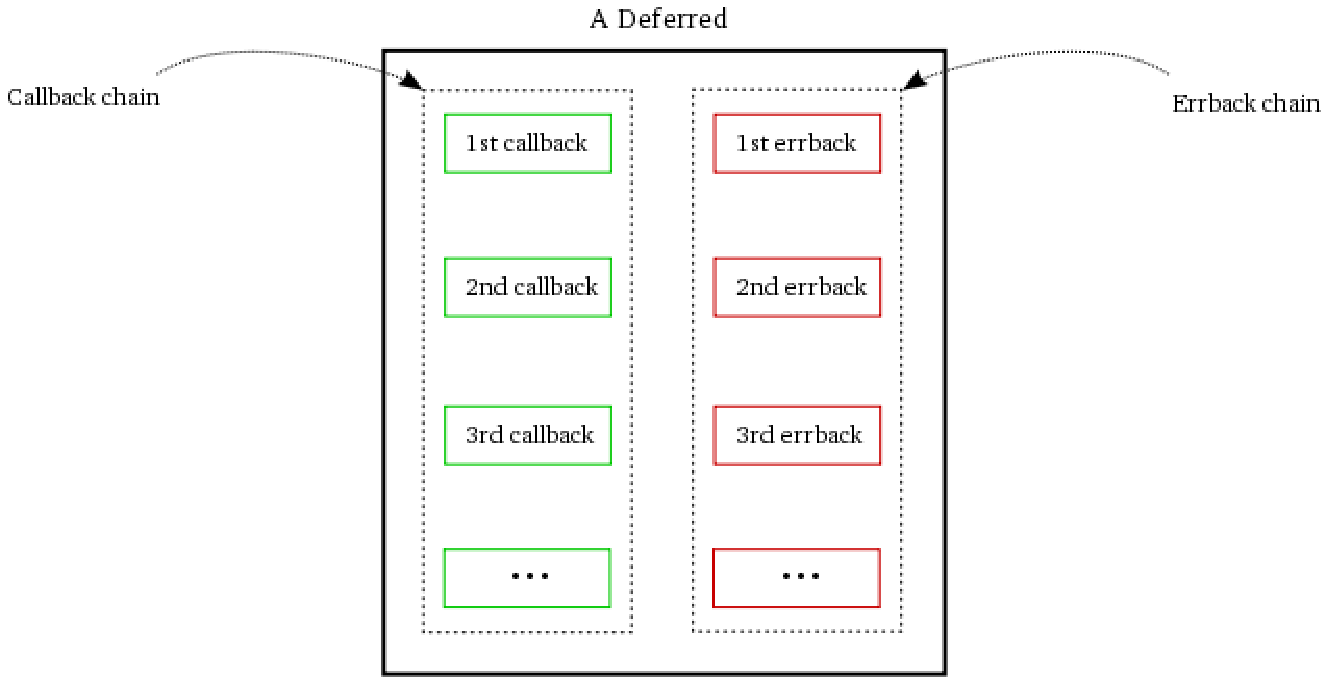
\includegraphics[width=0.8\textwidth]{images/deferred-1.pdf}
    \caption{Deferred\label{fig:deferred-1}}
\end{center}
\end{figure}

\eject

%Let’s try this out. Since deferreds don’t use the reactor, we can test them out without starting up the loop.
Давайте опробуем это. Поскольку deferred'ы не используют 
reactor, мы можем их попробовать, не запуская цикла.


%You might have noticed a method on Deferred called setTimeout that does use the reactor. It is deprecated and will cease to exist in a future release. Pretend it’s not there and don’t use it.
Вы могли бы заметить, что метод setTimeout класса Deferred 
использует reactor. Эта часть устарела, и, возможно, прекратит существовать 
в следующем релизе. Сделайте вид, что этого здесь нет и не 
используйте.


%Our first example is in twisted-deferred/defer-1.py:
Наш первый пример находится в 
\href{http://github.com/jdavisp3/twisted-intro/blob/master/twisted-deferred/defer-1.py}{twisted-deferred/defer-1.py}:

\begin{scriptsize}\begin{verbatim}
from twisted.internet.defer import Deferred

def got_poem(res):
    print 'Your poem is served:'
    print res

def poem_failed(err):
    print 'No poetry for you.'

d = Deferred()

# add a callback/errback pair to the chain
d.addCallbacks(got_poem, poem_failed)

# fire the chain with a normal result
d.callback('This poem is short.')

print "Finished"
\end{verbatim}\end{scriptsize}


%This code makes a new deferred, adds a callback/errback pair with the addCallbacks method, and then fires the “normal result” chain with the callback method. Of course, it’s not much of a chain since it only has a single callback, but no matter. Run the code and it produces this output:
Этот код создает новый deferred, добавляет пару callback/errback с 
методом addCallbacks, и затем активизирует цепочку с <<нормальным результатом>> 
с помощью метода callback. Запуститите код, и он напечатает следующее:

\begin{scriptsize}\begin{verbatim}
Your poem is served:
This poem is short.
Finished
\end{verbatim}\end{scriptsize}

%That’s pretty simple. Here are some things to notice:
Это достаточно просто. Вот, что стоит отметить:

\begin{enumerate}
%   1. Just like the callback/errback pairs we used in client 3.1, the callbacks we add to this deferred each take one argument, either a normal result or an error result. It turns out that deferreds support callbacks and errbacks with multiple arguments, but they always have at least one, and the first argument is always either a normal result or an error result.
\item Подобно парам callback/errback, которые мы использовали в 
клиенте 3.1, callback'и, которые мы добавили к этому deferred'у, 
берут в качестве аргумента либо нормальный результат, либо ошибку. 
Оказывается, что deferred'ы поддерживают callback'и и errback'и 
с несколькими аргументами, но они всегда имеют по меньшей мере 
один аргумент: нормальный результат или результат с ошибкой.

%   2. We add callbacks and errbacks to the deferred in pairs.
\item Мы добавляем callback'и и errback'и в deferred парами.

%   3. The callback method fires the deferred with a normal result, the method’s only argument.
\item Метод callback активизирует deferred с нормальным результатом, 
единственным аргументом метода.

%   4. Looking at the order of the print output, we can see that firing the deferred invokes the callbacks immediately. There’s nothing asynchronous going on at all. There can’t be, since no reactor is running. It really boils down to an ordinary Python function call.
\item Смотря на порядок вывода print'а, можно заметить, 
что активизация deferred'а вызывает callback'и немедленно. 
Здесь нет ничего асинхронного и не могло бы быть, поскольку 
reactor не запущен. Это реально сводится к обычному вызову 
функции в Python'е.

\end{enumerate}

%Ok, let’s push the other button. The example in twisted-deferred/defer-2.py fires the deferred’s errback chain:
Хорошо, давайте нажмем на другую кнопку. Пример в 
\href{http://github.com/jdavisp3/twisted-intro/blob/master/twisted-deferred/defer-2.py}{twisted-deferred/defer-2.py} 
активизирует errback цепочку deferred'а:

\begin{scriptsize}\begin{verbatim}
from twisted.internet.defer import Deferred
from twisted.python.failure import Failure

def got_poem(res):
    print 'Your poem is served:'
    print res

def poem_failed(err):
    print 'No poetry for you.'

d = Deferred()

# add a callback/errback pair to the chain
d.addCallbacks(got_poem, poem_failed)

# fire the chain with an error result
d.errback(Failure(Exception('I have failed.')))

print "Finished"
\end{verbatim}\end{scriptsize}

%And after running that script we get this output:
После запуска этой программы, мы получим вывод:

\begin{scriptsize}\begin{verbatim}
No poetry for you.
Finished
\end{verbatim}\end{scriptsize}


%So firing the errback chain is just a matter of calling the errback method instead of the callback method, and the method argument is the error result. And just as with callbacks, the errbacks are invoked immediately upon firing.
Таким образом, активизация цепочки errback состоит только в 
вызове метода errback вместо callback, где в качестве 
аргумента использовали результат с ошибкой. Также как с 
callback'ми, errback'и вызываются сразу же после активизации.  


%In the previous example we are passing a Failure object to the errback method like we did in client 3.1. That’s just fine, but a deferred will turn ordinary Exceptions into Failures for us. We can see that with twisted-deferred/defer-3.py:

В предыдущем примере мы передаем объект Failure к методу 
errback подобно тому, как мы делали это в клиенте 3.1. Это отлично, 
но deferred обертывает для нас обычные Exception в Failure. Мы 
можем увидеть это в 
\href{http://github.com/jdavisp3/twisted-intro/blob/master/twisted-deferred/defer-3.py}{twisted-deferred/defer-3.py}:

\begin{scriptsize}\begin{verbatim}
from twisted.internet.defer import Deferred

def got_poem(res):
    print 'Your poem is served:'
    print res

def poem_failed(err):
    print err.__class__
    print err
    print 'No poetry for you.'

d = Deferred()

# add a callback/errback pair to the chain
d.addCallbacks(got_poem, poem_failed)

# fire the chain with an error result
d.errback(Exception('I have failed.'))
\end{verbatim}\end{scriptsize}


%Here we are passing a regular Exception to the errback method. In the errback, we are printing out the class and the error result itself. We get this output:
Здесь мы подставляем обычный Exception в метод errback. 
В errback'е, мы печатаем класс и сам результат. Мы получаем такой вывод:

\begin{scriptsize}\begin{verbatim}
twisted.python.failure.Failure
[Failure instance: Traceback (failure with no frames): : I have failed.
]
No poetry for you.
\end{verbatim}\end{scriptsize}


%This means when we use deferreds we can go back to working with ordinary Exceptions and the Failures will get created for us automatically. A deferred will guarantee that each errback is invoked with an actual Failure instance.
Это означает, что когда мы используем deferred'ы, мы можем 
вернуться обратно к работе с обычными исключениями, и объекты 
типа Failure создадутся для нас автоматически. deferred будет 
гарантировать, каждый errback вызывается с действительным 
экземпляром Failure.


%We tried pressing the callback button and we tried pressing the errback button. Like any good engineer, you probably want to start pressing them over and over. To make the code shorter, we’ll use the same function for both the callback and the errback. Just remember they get different return values; one is a result and the other is a failure. Check out twisted-deferred/defer-4.py:
Мы попробовали нажать на кнопку callback, и 
мы попробовали нажать на кнопку errback. Подобно любым 
хорошим инженерам, вы вероятно хотите нажать еще раз. 
Чтобы сделать код короче, мы будем использовать ту же 
функцию для обоих callback и errback. Только запомните, что 
они получают различные возвращаемые значения: один - результат, 
другой - ошибка. Посмотрите 
\href{http://github.com/jdavisp3/twisted-intro/blob/master/twisted-deferred/defer-4.py}{twisted-deferred/defer-4.py}:

\begin{scriptsize}\begin{verbatim}
from twisted.internet.defer import Deferred
def out(s): print s
d = Deferred()
d.addCallbacks(out, out)
d.callback('First result')
d.callback('Second result')
print 'Finished'
\end{verbatim}\end{scriptsize}

%Now we get this output:
Теперь мы получаем этот вывод:

\begin{scriptsize}\begin{verbatim}
First result
Traceback (most recent call last):
  ...
twisted.internet.defer.AlreadyCalledError
\end{verbatim}\end{scriptsize}


%This is interesting! A deferred will not let us fire the normal result callbacks a second time. In fact, a deferred cannot be fired a second time no matter what, as demonstrated by these examples:
Это интересно! deferred не позволяет нам 
активизировать нормальный результат во второй раз. 
Фактически, deferred не может быть активизирован во второй 
раз, что демонстируется в следующих примерах: 

\begin{itemize}
\item \href{http://github.com/jdavisp3/twisted-intro/blob/master/twisted-deferred/defer-4.py}{twisted-deferred/defer-4.py}
\item \href{http://github.com/jdavisp3/twisted-intro/blob/master/twisted-deferred/defer-5.py}{twisted-deferred/defer-5.py}
\item \href{http://github.com/jdavisp3/twisted-intro/blob/master/twisted-deferred/defer-6.py}{twisted-deferred/defer-6.py}
\item \href{http://github.com/jdavisp3/twisted-intro/blob/master/twisted-deferred/defer-7.py}{twisted-deferred/defer-7.py}
\end{itemize}


%Notice those final print statements are never called. The callback and errback methods are raising genuine Exceptions to let us know we’ve already fired that deferred. Deferreds help us avoid one of the pitfalls we identified with callback programming. When we use a deferred to manage our callbacks, we simply can’t make the mistake of calling both the callback and the errback, or invoking the callback twenty-seven times. We can try, but the deferred will raise an exception right back at us, instead of passing our mistake onto the callbacks themselves.
Заметьте, что последние операторы print никода не вызовутся. 
Методы calback и errback вызывают исключения, 
чтобы дать нам понять, что мы уже активизировали этот deferred. 
Deferred'ы помогают нам избежать ловушек, которые мы идентифицировали 
как повторный вызов. Когда мы используем 
deferred для управления нашими callback'ми, мы просто не можем 
сделать ошибку вызвав одновременно callback и errback, или вызывая callback 
27 раз. Мы можем попробовать, но deferred сгенерирует исключение, 
вместо того, чтобы подставить нашу ошибку в сами callback'и. 


%Can deferreds help us to refactor asynchronous code? Consider the example in twisted-deferred/defer-8.py:
Могут ли deferred'ы помочь нам улучшить асинхронный код? 
Рассмотрим пример в 
\href{http://github.com/jdavisp3/twisted-intro/blob/master/twisted-deferred/defer-8.py}{twisted-deferred/defer-8.py}:

\begin{scriptsize}\begin{verbatim}
import sys

from twisted.internet.defer import Deferred

def got_poem(poem):
    print poem
    from twisted.internet import reactor
    reactor.stop()

def poem_failed(err):
    print >>sys.stderr, 'poem download failed'
    print >>sys.stderr, 'I am terribly sorry'
    print >>sys.stderr, 'try again later?'
    from twisted.internet import reactor
    reactor.stop()

d = Deferred()

d.addCallbacks(got_poem, poem_failed)

from twisted.internet import reactor

reactor.callWhenRunning(d.callback, 'Another short poem.')

reactor.run()
\end{verbatim}\end{scriptsize}

%This is basically our original example above, with a little extra code to get the reactor going. Notice we are using callWhenRunning to fire the deferred after the reactor starts up. We’re taking advantage of the fact that callWhenRunning accepts additional positional- and keyword-arguments to pass to the callback when it is run. Many Twisted APIs that register callbacks follow this same convention, including the APIs to add callbacks to deferreds.
Код выше - это наш первоначальный пример, с 
дополнительным запуском реактора. Заметьте, 
что мы используем callWhenRunning для активизации deferred'а 
после запуска реактора. Мы пользуемся тем фактом, что 
\href{http://twistedmatrix.com/trac/browser/tags/releases/twisted-8.2.0/twisted/internet/interfaces.py#L766}{callWhenRunning} 
принимает дополнительные позиционные и ключевые (keyword) аргументы 
для того, чтобы подставить их в callback во время его запуска. 
Многие Twisted API, регистрирующие callback'и, следуют 
этому соглашению, включая API для добавления callback'ов в deferred'ы.


%Both the callback and the errback stop the reactor. Since deferreds support chains of callbacks and errbacks, we can refactor the common code into a second link in the chains, a technique illustrated in twisted-deferred/defer-9.py:
И callback, и errback останавливают reactor. 
Поскольку deferred'ы поддерживают цепочки 
callback'ов и errback'ов, мы можем улучшить общий код, 
создав вторую ссылку в цепочках, что проиллюстрировано в 
\href{http://github.com/jdavisp3/twisted-intro/blob/master/twisted-deferred/defer-9.py}{twisted-deferred/defer-9.py}:

\begin{scriptsize}\begin{verbatim}
import sys

from twisted.internet.defer import Deferred

def got_poem(poem):
    print poem

def poem_failed(err):
    print >>sys.stderr, 'poem download failed'
    print >>sys.stderr, 'I am terribly sorry'
    print >>sys.stderr, 'try again later?'

def poem_done(_):
    from twisted.internet import reactor
    reactor.stop()

d = Deferred()

d.addCallbacks(got_poem, poem_failed)
d.addBoth(poem_done)

from twisted.internet import reactor

reactor.callWhenRunning(d.callback, 'Another short poem.')

reactor.run()
\end{verbatim}\end{scriptsize}

%The addBoth method adds the same function to both the callback and errback chains. And we can refactor asynchronous code after all.
Метод addBoth добавляет одну и ту же функцию в обе цепочки 
callback и errback. И, в конце концов, мы можем улучшить асинхронный код.


%Note: there is a subtlety in the way this deferred would actually execute its errback chain. We’ll discuss it in a future Part, but keep in mind there is more to learn about deferreds.
Замечание: существует тонкость в способе, когда 
deferred действительно выполнял бы свою errback цепочку. 
Мы обсудим это в следующей главе, но запомните, что еще есть что 
изучить о deferred'ах.


\subsection{Резюме}

%In this Part we analyzed callback programming and identified some potential problems. We also saw how the Deferred class can help us out:
В этой главе мы анализировали программирование с использованием 
callback'ов и идентифицировали некоторые потенциальные проблемы. 
Мы также увидели, как класс Deferred может выручить нас в следующих 
ситуациях:

\begin{enumerate}
%   1. We can’t ignore errbacks, they are required for any asynchronous API. Deferreds have support for errbacks built in.
\item Мы не можем игнорировать errback'и, так как они требуются 
для любого асинхронного API. Deferred'ы имеют встроенную поддержку errback'ов.  

%   2. Invoking callbacks multiple times will likely result in subtle, hard-to-debug problems. Deferreds can only be fired once, making them similar to the familiar semantics of try/except statements.
\item Вызов callback'ов несколько раз может вызвать зависание программы, и 
это трудно отлаживать. Deferred'ы могут активизироваться только один 
раз, что делает их похожими на семантику оператора try/except.

%   3. Programming with plain callbacks can make refactoring tricky. With deferreds, we can refactor by adding links to the chain and moving code from one link to another.
\item Программирование с помощью обычных callback'ов делает 
рефакторинг сложным. С помощью deferred'ов, мы можем рефакторить, 
добавляя ссылки в цепочку и перемещая код из одной 
ссылки в другую.

\end{enumerate}

%We’re not done with the story of deferreds, there are more details of their rationale and behavior to explore. But we’ve got enough to start using them in our poetry client, so we’ll do that in Part 8.
Мы еще не завершили рассмотрение deferred'ов, так как существует 
большое количество деталей их обоснования и поведения. Но теперь 
мы имеем достаточно для того, чтобы начать использовать 
их в нашем поэтическом клиенте, и мы сделаем это 
в следующей главе.

\subsection{Упражнения}

\begin{enumerate}
%   1. The last example ignores the argument to poem_done. Print it out instead. Make got_poem return a value and see how that changes the argument to poem_done.
\item Последний пример игнорирует аргумент poem\_done. Распечатайте его. 
Сделайте так, чтобы got\_poem возвращал значение и посмотрите на изменения в 
аргументе poem\_done.

%   2. Modify the last two deferred examples to fire the errback chains. Make sure to fire the errback with an Exception.
\item Поменяйте два последних примера с deferred'ми и активизируйте errback цепочки. 
Убедитесь, что активизировали errback с Exception.  

%   3. Read the docstrings for the addCallback and addErrback methods on Deferred.
\item Прочитайте строки с документацией для методов addCallback и addErrback  
класса Deferred. 

\end{enumerate}
